\section{Design pattern}

\begin{frame}
    \frametitle{Refactoring with the strategy pattern}
    \vspace{-5pt}
    \textbf{Problem:} Methods for I/O and calculations will change frequently

    \vspace{-5pt}
    \textbf{Solution:} Implement strategy design pattern $\rightarrow$ Define a family of algorithms and encapsulate them

    \vspace{-5pt}
    \begin{columns}
        \begin{column}{0.5\textwidth}
            \begin{itemize}
                \item \textbf{Structure: } 
                \vspace{-5pt}
                \begin{itemize}
                    \item Simulation as the highest layer for choosing strategy
                    \item Compartmentalizing I/O, model and physics
                    \item Enabling Combinations of physics functions through strategy
                \end{itemize}
            \end{itemize}
        \end{column}
        \begin{column}{0.5\textwidth}
            \begin{itemize}
                \item \textbf{Benefits: }
                    \begin{itemize}
                        \item Simple swapping of algorithms
                        \item Isolation of implementation details
                        \item Open/Closed Principle: Introduction of new strategies without context change
                    \end{itemize}
            \end{itemize}
        \end{column}
    \end{columns}

    \begin{figure}
        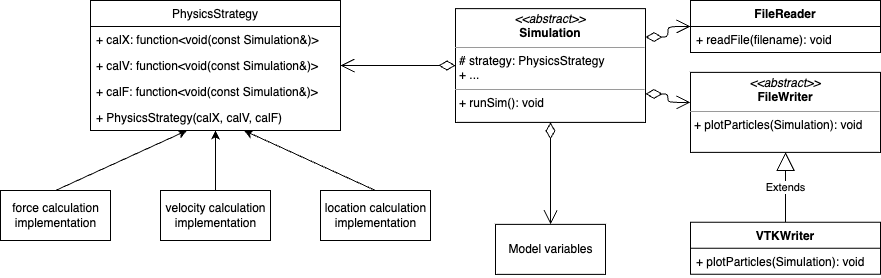
\includegraphics[width=.8\columnwidth]{../../../report/report1/res/strategy_long.png}
        \caption{UML-like diagram showing our implementation of the strategy pattern}
    \end{figure}

\end{frame}